\documentclass[12pt,letterpaper]{article}

\usepackage[hmargin=1in,bottom=1in,top=1in]{geometry}
\usepackage[latin1]{inputenc}
\usepackage{amsmath}
\usepackage{amsfonts}
\usepackage{amssymb}
\usepackage{graphicx}
\usepackage{url}
%\usepackage[toc,page]{appendix}
\usepackage{setspace}

\usepackage{ulem}
\normalem

% push footnotes to the bottom of the page unconditionally
\usepackage[bottom]{footmisc}

\usepackage[pdftex]{hyperref}
\hypersetup{
	pdfauthor={Neil Isaac and Keyi Shi},
	pdftitle={Implementation of a virtual FPGA architecture},
	pdfsubject={Virtual FPGA fabrics},
	colorlinks=true,
	anchorcolor=black,
	linkcolor=blue,
	citecolor=blue,
	filecolor=blue,
	pagecolor=blue,
	urlcolor=blue,
	frenchlinks=false,
	pagebackref=true,
	bookmarks=true}

% make links to figures jump to position above the figure
%\usepackage[all]{hypercap}

%\usepackage{titling}
%\usepackage{listings}
%\lstset{language=c}

% fancyhdr - use top=1.5in
%\usepackage{fancyhdr}
%\pagestyle{fancy}
%\fancyhead[L]{\leftmark}
%\fancyhead[R]{\thepage}
%\fancyhead[CF]{}
%\setlength{\headheight}{16pt}

\setlength{\parindent}{0in}
\setlength{\parskip}{1.0 \baselineskip}
\setlength{\footnotesep}{1.0 \baselineskip}
\setlength{\skip\footins}{2.0 \baselineskip}

\bibliographystyle{IEEEtran}

\usepackage{color}
\newcommand{\note}[1]{}
% comment out the next line to hide draft notes
\renewcommand{\note}[1]{\textcolor{red}{[#1]}}
\newcommand{\citationneeded}[0]{\note{citation needed}}

\newenvironment{enumeration}{
	\setlength{\topsep}{0.0pt}
	\setlength{\partopsep}{0pt}
	\setlength{\parskip}{0pt}
	\setlength{\parsep}{0pt}
	\begin{enumerate}
		\setlength{\itemsep}{0pt}}
	{\end{enumerate}}

\newenvironment{itemlist}{
	\setlength{\topsep}{0pt}
	\setlength{\partopsep}{0pt}
	\setlength{\parskip}{0pt}
	\setlength{\parsep}{0pt}
	\begin{itemize}
		\setlength{\itemsep}{0pt}}
	{\end{itemize}}

\newcommand{\sectref}[1]{section \ref{#1}}

%\renewcommand{\thefootnote}{\roman{footnote}}

\begin{document}

%\begin{titlepage}
\begin{center}


\includegraphics[scale=1.0]{ecelogo.png}

\vspace{1 \baselineskip}

\textsc{
\Large University of Toronto\\
\large Department of Electrical and Computer Engineering \\
\large ECE496 Design Project
}

\vspace{2 \baselineskip}

{\Large \bfseries Virtual FPGA fabrics} \\
{\Large \bfseries Implementation of a Virtual FPGA Architecture}

\vspace{2 \baselineskip}

{\large \bfseries Final Report} \\

\vspace{2 \baselineskip}

{\large March 22, 2012}

\vfill

\begin{tabular*}{4in}{l @{\extracolsep{\fill}} l}
\textbf{Neil Isaac} & \textbf{Keyi Shi} \\
\texttt{n.isaac@utoronto.ca} & \texttt{keyi.shi@utoronto.ca} \\ & \\
\emph{Project ID:} & 2011017 \\
\emph{Supervisor:} & Jason Anderson \\
\emph{Administrator:} & Ross Gillett \\
\emph{Section:} & \#7 \\
\end{tabular*}

\end{center}
\end{titlepage}



\onehalfspace

\thispagestyle{empty}
\section*{Executive Summary}

% No more than 1 page
% Should show clear understanding of AUDIENCE and PURPOSE
% Readable as a stand-alone document, clearly differentiated from an introduction
% Give the contest and MOST IMPORTANT information in the document in a unified fashion

Academic studies of Field Programmable Gate Array (FPGA) chip architecture rely on simulations, as commercial FPGA chips contain proprietary designs that make their underlying architecture inaccessible to academic researchers.
The goal of this project is to provide a physical platform for researchers to carry out FPGA architecture studies.
The finished design should capable of running common benchmark circuits.

The proposed design is to implement an Overlay FGPA on an existing, commercially available FPGA chip.
Using a commercial FPGA as the physical medium for this project makes the design cheaper and more accessible to researchers, as they may have an appropriate FPGA chip already.


We have selected the Xilinx Virtex 5 FPGA as our development platform because we can use its native logic units directly.
This will limit the models of FPGA chips that the overlay circuit can be implemented on, but it should reduce the design's area overhead and improve its timing characteristics.
The features we will use on the Virtex 5 are forward-compatible with all current-generation Xilinx FPGA products, allowing the researcher to use a variety of FPGAs.

The validation of the design will involve testing a set of benchmark circuits by placing and routing them with VPR, then transferring them to the FPGA overlay.
The circuits can then be tested for correct behavior, confirming that the overlay design can be correctly programmed using VPR output, and that the inputs and outputs to the design are functioning properly.

The current budget for the proposed design is \$14.00 and will be covered by the students.
The required FPGA development boards and software licenses have been provided by the supervisor.

We have designed and tested the modules required to build one tile of the Overlay FGPA.
By December, we expect to have assembled a grid of tiles and have software support for programming the logic cells.



\setcounter{tocdepth}{2}
\tableofcontents
%\listoffigures
%\listoftables
\pagebreak

\section{Project Description}

\subsection{Background and Motivation}

% This section is aimed at demonstrating your team's understanding of the technical
% problem and „the big picture‟. Provide a background, context [Design Notes, chapter 4]
% and motivation for your project. A good project is not following a recipe; what makes
% your project different than what is available? (Note that if the implementation of an
% existing product is not obvious and is not available, or can be done in an alternate way,
% then implementing would still make a reasonable project.)
%
% The work may just be an interesting exercise in technology, or may have direct or indirect
% practical application. It could improve reliability, cost, or ease of use over available
% technology. It may deal with some interesting challenges.
%
% Understanding the problem in the context of the bigger picture requires that you do a
% literature search, and you should be prepared to put in enough time to build your case.
% Provide relevant references to original sources of information. References to webpages
% (like Wikipedia) are generally inadequate, unless they can be justified (e.g. datasheet for
% components). Wherever possible, reference original sources such as journals, books, and
% technical standards, and provide complete information in a standard format (Refer to
% examples from IEEE on the course website.)
%
% Previous Background Work (if applicable)
% Many uncertainties about risks are answered in the course of working on a problem. In
% this respect, groups that have actively worked on their project over the summer have a
% key advantage, and so should briefly highlight some of the key challenges they have
% already overcome. Evidence here provides strong support of the feasibility of the
% remainder of the project. These groups can include some of their previous work as an
% attachment in the appendix.

Academic researchers who study Field Programmable Gate Array (FPGA) design commonly use variations of an FPGA design architecture, described by Kuon et al\cite{fpga}, which we will refer to as the \emph{Academic FPGA Model}.
While FPGA chips are available from a variety of commercial vendors, their design is largely proprietary, making their architectures difficult to study.\citationneeded
Furthermore, there is no existing physical implementation\footnote{Alex Brant is also developing a comparable FPGA overlay platform with Prof. Guy Lemieux at University of British Columbia.} of an Academic FPGA Model.

One of the tools used in FPGA architecture research is VPR\cite{vpr}.
VPR is a free, open-source placement and routing tool that accepts a wide variety of architecture parameters. \citationneeded
It is not currently possible to realize VPR output on a commercial FPGA.\footnote{A technology-mapped input netlist for VPR can be converted to an Altera Quartus VQM netlist file using \emph{nettovqm}\cite{nettovqm}, but the placement and routing can not be converted.}

As such, Computer Aided Design (CAD) researchers who work on placement and routing algorithms for FPGA designs are presently limited to using simulations to evaluate or verify their work.
They may be interested in testing circuit realizations on a physical medium.



\subsection{Project Goal}

% The project goal is a statement that summarizes what your design project is to achieve. It
% can be general and non-technical but should give direction to the entire project. It is NOT
% just the statement your supervisor used to describe the project. Refer to [Design, Section
% 3.2] to find both good and bad examples of project goal statements. Two key points are to
% focus on the desired result, not the solution or implementation, and to establish some
% criteria for which the success of the project can be evaluated.
% 
% Design projects can take many forms. There are those that have hard functional goals but
% the details of the methodology are left undefined. An example of this type is the building
% of a microprocessor simulator. Another type, common to research-oriented projects, is a
% feasibility study or experiment where the result of the study is not known; however the
% setup of the study is a hard functional goal. Such projects may be somewhat harder to
% define but must meet the same requirements for verifiable project goals. One aid in these
% cases is to think of what has to be specified to guarantee that another team could exactly
% duplicate the experiment.

The goal of this project is to produce a circuit design based on the Academic FPGA model.
Researchers will be able to use the circuit to study FPGA architecture and CAD algorithms with circuits produced by VPR.



\subsection{Project Requirements}

% Provide a list of target project requirements which will be used to evaluate the success of
% your project. Project requirements can be divided into three categories [Design Notes,
% Section 5.2]:
% - Functional requirements
% - Constraints
% - Objectives
%
% Functional requirements and constraints should be clearly worded in pass/fail terms
% and in a way that can be verified, which implies a corresponding set of verification tests
% will be needed as discussed in the next section. Project objectives, unlike functional
% requirements and constraints, are not intended to be pass/fail in nature, but are used to
% indicate the desirable aspects of the final design. The number of requirements depends
% largely on the project, but at this early stage, the list should not be very long, but enough
% to capture the essence of your project. The point is to be complete, but not to constrain
% your design unnecessarily. Use the Requirements Checklist in [Design Notes, Section
% 5.4] to guide you.


\subsubsection{Functional Requirements}

Researchers must be able to:
\begin{itemlist}
	\item implement the overlay FPGA circuit on commercially available FPGA chips,
	\item tune the number, arrangement, and logic cell connectivity of the overlay FPGA,
	\item program the overlay FPGA using an output circuit from VPR,
	\item modify the inputs and outputs of the overlay FPGA.
\end{itemlist}


\subsubsection{Constraints}

\begin{itemlist}
	\item The overlay circuit must support at least 3000 logic cells\footnote{3000 logic cells was choosen as the minimum target because the largest of the ``Golden 20'' circuits, \emph{``s38417''} requires 2567 6-input logic cells\cite{synthesis-density}.} in order to accommodate the \emph{``Golden 20''} MCNC benchmark circuits\footnote{The ``Golden 20'' MCNC circuits are available in BLIF format at \url{http://www.ece.ubc.ca/~julienl/benchmarks.htm}.} commonly used in FPGA research.
\end{itemlist}


\subsubsection{Objectives}

\begin{itemlist}
	\item Be compatible with accessibly priced commercial FPGAs.
	\item Take advantage of the underlying FPGA architectural features in the overlay FPGA design to reduce area and latency.
\end{itemlist}


\subsection{Validation and Acceptance Tests}

% In this section, describe how you would validate your final design and prove that it
% satisfies the project goal and requirements [Design Notes, Chapter 13]. Consider how you
% would demonstrate your successful project at the final Design Fair. Alternatively, if you
% were the paying client, describe the tests you would perform to qualify this product
% before buying this product. Provide details where possible, including the test equipment,
% diagnostic software, special arrangements, or test “jigs” that might be required. If you
% will be doing statistical measures, indicate the number of samples you will test. The point
% here is to keep your end goal in mind right from the start of the project.

\subsubsection{Functional validation}

To ensure that the overlay FPGA circuit design is functional, we will:
\begin{enumeration}
	\item select and use a benchmark circuit commonly used to test VPR,
	\item configure VPR to match our architecture and dimensions,
	\item place and route the benchmark circuit with VPR,
	\item convert the VPR output into a bitstream for the overlay FPGA,
	\item load the bitstream onto the overlay FPGA, then 
	\item test the functionality of the benchmark circuit running on the overlay FPGA.
\end{enumeration}
This test procedure ensures that:
\begin{itemlist}
	\item circuits can be implemented using VPR output,
	\item circuits can be transferred correctly to the overlay FPGA, and
	\item inputs can be set and outputs can be read.
\end{itemlist}
The exact verification process for inputs and outputs will depend on the benchmark circuit's intended function.
We will need to develop an appropriate testing mechanism for the benchmark circuit.


\subsubsection{Size and overhead validation}

To ensure that the overhead is low enough that the overlay FPGA can fit useful circuits, we will test it using the \emph{``Golden 20''} MCNC benchmark circuits.
For each circuit, we will:
\begin{enumeration}
	\item run synthesis and technology mapping using ABC,
	\item run placement and routing using VPR configured, and
	\item confirm that VPR can place and route the benchmark circuit using the number and arrangement of logic blocks that we can fit.
\end{enumeration}
We discuss risk mitigation for high overhead in \sectref{risk-size}.


\subsubsection{Validation of improvements from architectural optimizations}

To evaluate the benefits of utilizing architectural FPGA features of the host FPGA board, an alternate design can be created that implements the same functionality using only standard verilog.
The size and timing of the two designs can then be compared to measure any efficiency gained by the design that uses special FPGA features.

For example, in select Xilinx boards, a lookup table can be used as a 32-bit shift register; the same function could be implemented in plain Verilog using multiplexers and flip-flops, but is expected to be slower and consume more area.
The two equivalent circuits can be compiled separately in order to compare their resource use and limiting timing path.
Because the utilization of architectural features limit the design to specific board families, they must be shown to enhance the circuit efficiency of this project in order to justify their use.


\section{Technical Design}

\subsection{Design Alternatives}

% In this section, you explore and discuss different possible solutions and design
% alternatives. Exploring possibilities is often neglected by designers eager to start on the
% first idea that comes to mind. Often, however, the first solution isn‟t the best. For
% instance, you may have in mind an implementation using a keyboard, but when you work
% back to the requirements you may realize that it is only the user control aspect that is
% required, and thus you can do it all from the attached personal computer. The key to
% designing is coming up with alternatives, and it is in exploring alternatives that you come
% to appreciate the inevitable design trade-offs that you will face.
% 
% DO NOT ESTABLISH A DESIGN CHOICE, AND THEN THINK ABOUT
% ALTERNATIVES JUST TO GET THIS DOCUMENT DONE.
% 
% Some alternatives may differ only in small variations in implementation, others may be
% quite different. You should provide enough of an evaluation of each choice to justify your
% selection of the proposed solution. Provide a preliminary assessment of the different
% design alternatives in terms of the project goal and requirements you've laid out. Create a
% comparison table if necessary [See Design Notes, Chapter 9 for more ideas].
% 
% You may find that this section and the next naturally collapse into a single section, or that
% you wish to keep them separate.

\subsubsection{Implementation medium}

The implementation medium for our circuit is a major decision impacting how accessible our circuit will be to researchers.
The main criteria are cost, size, and ease of use.
The lower the cost of the finished design to the researcher, the better.
We must also ensure that the design is large enough to handle circuits the researchers wish to test.
Finally, we want to make interfacing with the design's inputs and outputs as simple as possible.
The alternatives are as follows:

\begin{enumeration}
\item Custom integrated circuit \
	\begin{itemlist}
		\item Faster, smaller and more power efficient.
		\item High design and manufacturing costs.
		\item Lengthy design and manufacturing time-line.
		\item Once built, the parameters can't be modified without manufacturing a new chip.
		\item Inputs and outputs will require extra circuitry to interface with the circuit.
	\end{itemlist}
\item Overlay FPGA implemented on commercial FPGA \
	\begin{itemlist}
		\item Researchers may already own a compatible FPGA so they won't need to purchase new hardware.
		\item Using an FPGA allows the researcher to implement a virtual circuit to interface with the overlay FPGA.
		\item Need to pick a FPGA platform to target:
		\begin{enumeration}
			\item Basic FPGA without using architecture-specific features
				\begin{itemlist}
					\item Circuit will work on most FPGAs from most vendors, so it is the most widely accessible.
					\item Can't use architecture-specific features to save area and gain performance.
				\end{itemlist}
			\item Xilinx Virtex 5 or newer \
				\begin{itemlist}
					\item Lookup tables can be programmed directly as 32-bit shift registers.
					\item Large FPGAs with 330,000 logic cells for Virtex 5\cite{xilinx-virtex5} will fit a larger overlay circuit. Virtex 6 and 7 feature up to 760,000 and 2,000,000 logic cells respectively\cite{xilinx-models}.
					\item Higher cost for researchers.
				\end{itemlist}
			\item Xilinx Spartan 6 \
				\begin{itemlist}
					\item Lookup tables can be programmed directly as 32-bit shift registers.
					\item Smaller FPGA with 150,000 logic cells\cite{xilinx-models}, allowing smaller overlay circuit.
					\item Lower cost than Virtex 5.
				\end{itemlist}
			\item Altera Stratix IV or newer
				\begin{itemlist}
					\item Higher cost than Xilinx Spartan FPGAs.
					\item Large FPGAs with up to 820,000 logic cells for Stratix IV\cite{altera-stratix4} and up to 952,000 for Stratix V\cite{altera-stratix5}.
					\item Features a similar 32-bit shift register, but it isn't directly compatible with the Xilinx boards.
				\end{itemlist}
		\end{enumeration}
	\end{itemlist}
\end{enumeration}

Developing a custom integrated circuit is far too costly and time consuming for the scope of this project.
It was explored as an alternative to illustrate the necessity of targeting an existing FPGA.
We have tentatively selected the Virtex 5 FPGA because our supervisor has numerous development boards and software licenses readily available.
We also intend to use the 32-bit shift register functionality that is available in logic blocks in Virtex 5 and newer FPGAs.
This feature will allow us to reduce the overhead of the overlay FPGA circuit by directly using the native FPGA's features.
This selection limits the use of our circuit to modern Xilinx FPGAs including Spartan 6, Artix 7, Kintex 7, and Virtex 5, 6 and 7.



\subsubsection{Configuration mechanism}

Various parameters of our circuit, including the number, arrangement, and connectivity of the logic cells will be tunable.
There are two alternatives for the implementation of the configuration mechanism:
\begin{enumeration}
	\item Parameterized Verilog \
		\begin{itemlist}
			\item Requires the user to modify values within the Verilog source.
			\item Involves more complex Verilog code to accommodate flexible parameters.
		\end{itemlist}
	\item Software front end to generate Verilog code \
		\begin{itemlist}
			\item The generation software would be easier to use than modifying Verilog code.
			\item Front end code will be easier to write than parameterized Verilog.
			\item User may need to install a compiler or interpreter to run the software.
		\end{itemlist}
\end{enumeration}

We have tentatively decided to use parameterized Verilog because we deemed that the complexity of the configuration in our present design concept does not warrant a front end code generator.
If added features or a reevaluation of the design add configuration complexity, we may reconsider this, as this decision could be changed without revising a great deal of work.



\subsection{Assessment of Proposed Design} % for Draft B

% Comment about the strengths, weaknesses, and trade-offs made in the proposed solution.
% What reasons led you to choose this solution over some of the others you explored? This
% section does not need to be long, but ensures that you can provide some justification for
% your design decisions to date.

The decision to take advantage of the custom 32-bit shift registers in implementing our design entails the following trade-offs versus using only basic Verilog logic:
\begin{itemlist}
	\item The design is more efficient area and timing-wise.
	\item The data describing the circuit (known as the \emph{bitstream}) which is needed to program the design will be larger.
	\item The maximum size of the design will be limited by the amount of 32-bit shift registers available on the FPGA board, as opposed to the amount of flops.
	\item The design will be incompatible with boards that do not have custom 32-bit shift registers
\end{itemlist}

We have decided that performance efficiency outweighs the negative aspects of the larger bitstream and limitation of implementation platforms.
If the design is successful, adaptations can be made in the future to support the implementation of the design on more FPGA boards.



\subsection{System-level overview} % for final proposal
\label{system-overview}

\figref{module-diagram} shows the high-level interactions of the components used in our project.
The rectangles show software components, the circles show intermediate products or interfaces, and the parallelograms show primary inputs and outputs.
The components we are producing directly are contained within the dotted lines.

\begin{figure}[!h]
	\centering
	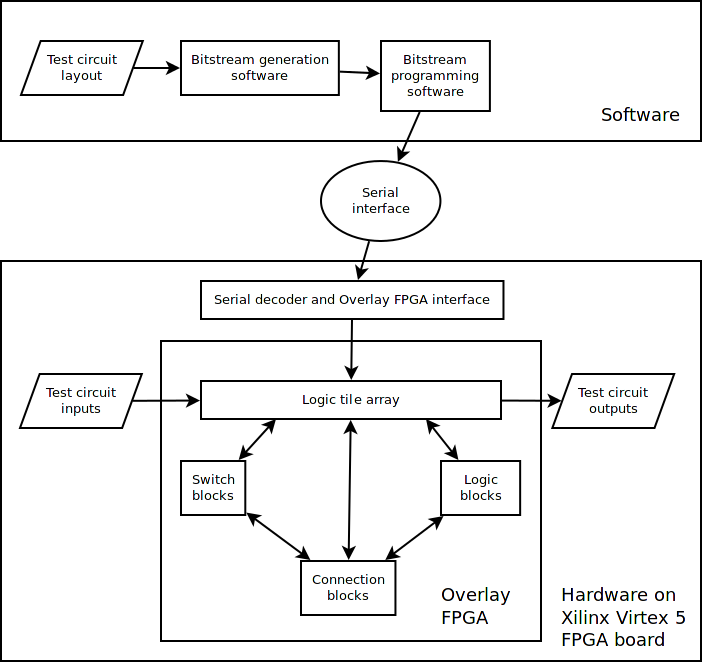
\includegraphics[scale=0.6]{modules.png}
	\caption{Module interaction}
	\label{module-diagram}
\end{figure}

The finished project will consist of three main parts: The overlay FPGA, bitstream generation software, and interfacing of inputs/outputs of the overlay FPGA.

The \emph{Overlay FPGA} is a Verilog HDL circuit implementation of the academic FPGA model which will be constructed as an overlay on a Xilinx FPGA board.
The arrangement, size and connectivity of the overlay circuit will be controllable via parameters in the source Verilog.
The overlay FPGA will consist of organized tiles of \emph{logic block}, \emph{connection block}, and \emph{switch block} modules.
Together, these modules will allow the overlay FPGA to implement different logic circuits.

Once built, the overlay FPGA can be configured to implement user-specified \emph{test circuits} that have been placed and routed by VPR.
This will be achieved by creating \emph{bitstream generation and programming software} that will translate the VPR output circuit into a bitstream that the overlay FPGA will understand.
The bitstream will then be injected into the overlay FPGA via a \emph{serial interface}.
The FPGA will receive and decode the bitstream into the appropriate test circuits on the overlay.

Finally, the circuits on the overlay FPGA can be tested for functionality by connecting devices (e.g. Switches and LEDs) to the \emph{Test circuit inputs} and \emph{Test circuit outputs} of the Overlay FPGA.


\subsection{Module-level descriptions} % for final proposal

The \emph{Overlay FPGA} will be composed of \emph{Logic tiles}.
The logic tiles make it easier to build a large overlay, and help keep the internal 
logic modules organized.
Each logic tile will consist of one \emph{logic block module}, two \emph{connection block modules}, 
and one \emph{switch block module}.
\figref{tile-diagram} shows the internal composition of a single logic tile.

\begin{figure}[!h]
	\centering
	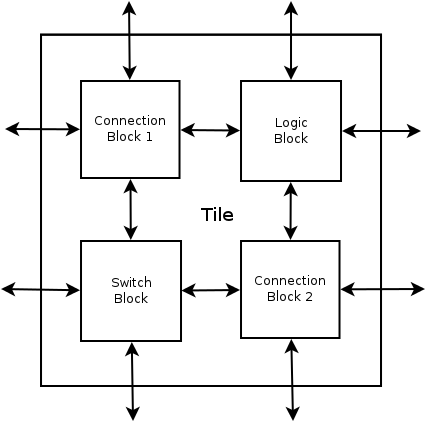
\includegraphics[scale=0.6]{tile.png}
	\caption{Logic connections within a tile}
	\label{tile-diagram}
\end{figure}

The \emph{Logic block module} consists of programmable look-up tables that perform all of the logical 
funcionality required by the circuit.
A logic block module may be composed of multiple look-up tables, the number of which 
can be determined by verilog parameters.

The \emph{Connection block} and \emph{Switch block} modules regulate the routing of signals in the overlay.
\emph{Connection blocks} connect logic block signals to buses that run throughout the 
overlay.
\emph{Switch blocks} control the routing between buses when they cross each other.

The \emph{Bitstream generation software} will be a program that translates VPR output circuits into a 
bitstream capable of programming the overlay FPGA directly.
The program will consist of functions that parse the output from VPR and generate the 
appropriate bitstream from the parsed information.

The \emph{Bitstream programming software} will take the bitstream formed by the bitstream generator 
and format it for proper transmission over a serial interface.

The \emph{Serial decoder} will be a circuit attached to the overlay FPGA that receives the 
bitstream sent through the serial interface.
It will decode and extract the bitstream 
from the serial format, then inject it into the overlay circuit to configure the 
overlay.



\section{Work plan}

%\subsection{Work breakdown structure} % for Draft B

%\subsection{Gantt chart} % for Draft B

%\subsection{Financial plan} % for Draft B

\subsection{Feasibility Assessment}

% This section is meant to help your team, supervisor, and administrator assess the
% feasibility of your proposed project. This is not a marketing exercise: try to provide a fair
% and honest assessment of your proposal, balancing both its strengths and weaknesses.
% There is nothing wrong with identifying major deficiencies in your project; in some
% businesses, fewer than one in ten projects results in a commercially viable product.
% Identifying weaknesses and putting together a plan to address those weaknesses early on
% is a crucial part of the design process. It also helps your supervisor and administrator in
% their roles as effective mentors and guides.
% 

% Here are some of the key issues you should address in this section. Be brief - a sentence
% or two is probably enough to cover each issue. Also, these issues do not need to be
% addressed in any particular order and may be combined or reorganized to flow logically:
% Skills and resources:
% - What are the key skills, knowledge and resources you need for this project?
% - What portions have you already acquired and what portions are currently lacking?
%   How do you plan to obtain what you still need? Examples:
%    o From the web: free or open source software, technical standards, expert
%      forums
%    o From your supervisor: graduate researchers, lab space and equipment, etc.
%    o From the Design Centre (SFB520): facilities for making and soldering
%      printed circuit boards, used hardware from past design projects,
%      computers, test equipment, etc.

\subsubsection{Skills and Resources}

\begin{itemlist}
	\item Required Software \
		\begin{itemlist}
			\item ABC synthesis system - available online\footnote{ABC can be downloaded from: http://www.eecs.berkeley.edu/~alanmi/abc/}
			\item VPR placement and routing - available online\footnote{VPR 5.0.2 can be downloaded from: http://www.eecg.utoronto.ca/vpr/}
			\item Vendor FPGA tools: Xilinx ISE - licenses from supervisor
		\end{itemlist}
	\item Required Hardware \
		\begin{itemlist}
			\item FPGA development board - currently using Xilinx Virtex 5 from supervisor.
We can discuss with our supervisor the possibility of getting alternate boards should the need arise.
			\item Host computer - personal laptops
			\item Serial cable and USB adapter - widely available at electronics stores at low prices
		\end{itemlist}
	\item Required Skills and Knowledge \
		\begin{itemlist}
			\item Verilog circuit design skilsl - gained from previous coursework and PEY experiences
			\item Knowledge of FPGA architecture - consulting with supervisor and studying recommended resources
			\item VPR interfacing - consulting with graduate students
		\end{itemlist}
\end{itemlist}


%
% Risk Assessment:
% In this section, describe the risks that the project could face (risk identification) and how
% you plan to deal with them (risk mitigation). An example of a risk would be that a
% particular component you envision might prove impossible to implement, and a
% corresponding risk mitigation strategy would be attempting to prototype the riskiest
% portion of your project as a feasibility assessment of the whole project. This would be
% coupled with a „fall-back‟ plan as to what you would do should this prototype fail.
% Merely, stating that risks will not occur, or that risks will be mitigated by working harder
% does NOT constitute back-up plan!
% This section should not be very long and you should focus on one or two real risks to
% your project (most likely technical risks but there could be others as well). Minor risks
% that will cause little disruption in schedule do not need to be addressed. Note that
% something that is technically challenging (or difficult to implement) may not necessarily
% be a significant risk to the project, if its failure does not affect the overall project goals or
% requirements (for example, the task may relate to a project objective for an additional
% feature, rather than a core requirement).
% Note: when addressing risks, focus on the most likely ones that are specific to your
% project. Some students ponder the risks of having a team member drop out of school, or
% losing all their work due to a computer crash. Such discussions aren't particularly helpful
% in planning your project. A more specific and effective series of questions might be
% - What happens to other components and to the project if component X that I‟ve
%     designed for my system fails to meet specifications or takes significantly longer to
%    develop?
% - Can I change the specifications, demonstrate a lower performance system, or
%   remove some features of my final design and still maintain the essential aspects of
%  my project?
% - What if our initial plan to build a real prototype proves unfeasible? Could we
%   demonstrate our design or part of our design using a computer model instead?
%  What would the limitations of this computer model-based prototype be? How
% would the project goal, requirements, and scope be modified to ensure that the
% new, redefined, project remains challenging?
% The key idea is to think of ways that you can modify the scope of your project so that you
% can show some partial success in realizing your Project Proposal by the end of the school
% year. More information and additional examples in [Design Notes, Chapter 11].
%
% Risk in Research Projects: Often, a research project will have above-average risk and
% this section may need to be longer. If the „Technical Design‟ section describes your
% intended initial strategy, this section should describe alternate directions that will be
% taken if experimental results indicate that the initial strategy is no longer what should be
% done. Here, the „risk‟ is that the experimental result or some intermediate result not be as
% expected (and the probability of this could be high) and the mitigation is the
% determination of an the alternate goal or an alternate route to the original goal.



\subsubsection{Risk Assessment}

\begin{itemlist}
	\item FPGA Size \
		\begin{itemlist}
			\item The circuit design may have too much overhead, making it impossible to fit on the selected FPGA board.
			\item Risk Mitigation: calculate circuitry resources needed for the overall design, and compare to resources available.
If it's insufficient, either a larger FPGA board must be chosen, or the circuit design needs to be re-done.
		\end{itemlist}
	\item Timing \
		\begin{itemlist}
			\item Timing on signals travelling between logic blocks may be unbalanced, as in the overlay logically adjacent cells may not be physically adjacent.
			\item Risk Mitigation: Design a rectangular "tile" containing only one logic block, and tesselate it to create the overall layout to keep timing consistent.
		\end{itemlist}
\end{itemlist}



\pagebreak
%\nocite{*} % show uncited entries in the bibliography
\bibliography{ref}
\addcontentsline{toc}{section}{References}

%\pagebreak
%\begin{appendices}
%\input{file}
%\include{file}
%\end{appendices}

%\pagebreak
%\fancyhead[L]{Addenda}
%\addcontentsline{toc}{section}{Title}
%\section*{Title}
%\input{file}
%\pagebreak

\end{document}

